\subsection{Verilog Designs \& Port Constraints}

\subsubsection{Music Player}

\defverbatim[colored]\musicmodule{
\begin{lstlisting}[language=verilog]
module musicplayer(
           input clk,
           input music_sel,
           input music_en,
           output reg music_frac_ext = 0
       );
\end{lstlisting}
\begin{itemize}
	\item<0-> clk: port Y18 (板载时钟, 100MHz)
	\item<0-> music\_sel: controlled by the main module
	\item<0-> music\_en: bgm on/off, controlled by a switch
	\item<0-> music\_frac\_ext: port A19 (蜂鸣器)
\end{itemize}
}

\begin{frame}{Music Player: IO ports}
	\musicmodule
\end{frame}


\begin{frame}{Music Player: How does it work?}
	\hspace{1em}
    \begin{column}<0->{.5\textwidth}
		\centerline{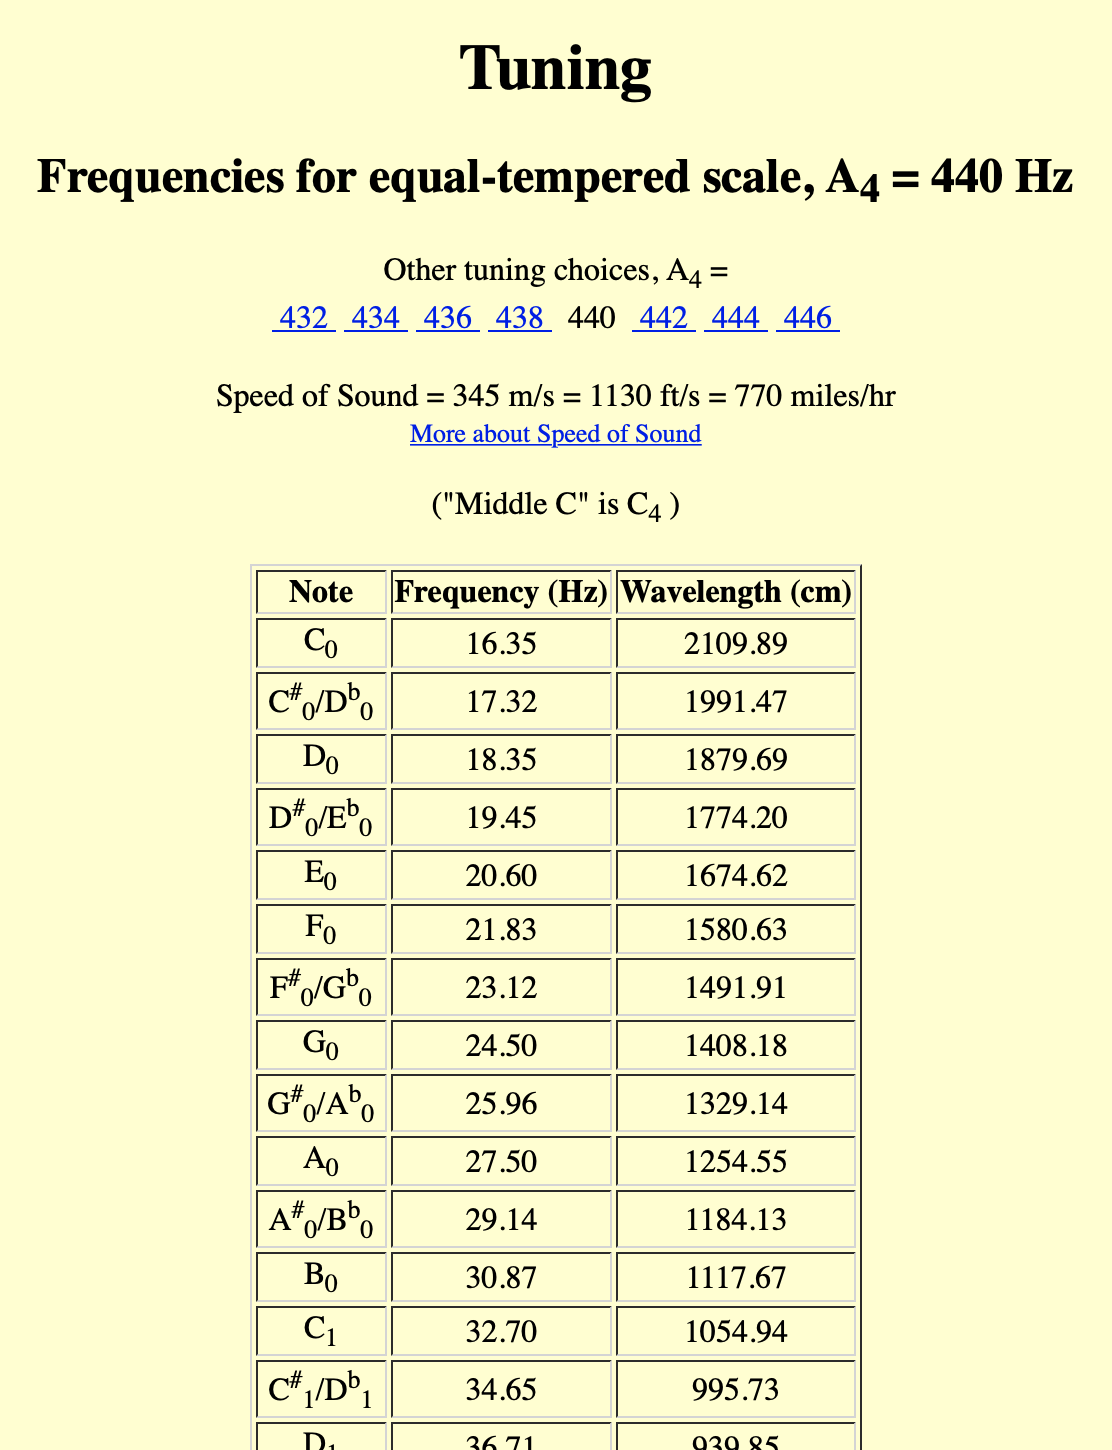
\includegraphics[height=5cm]{fig/music_hz}}
		\tiny
		\centerline{Retrieved from https://pages.mtu.edu/\%7Esuits/notefreqs.html}
		\normalsize
	\end{column}%

	\hfill%
	\begin{column}<0->{.5\textwidth}
		\vspace{-16.5em}
        \centerline{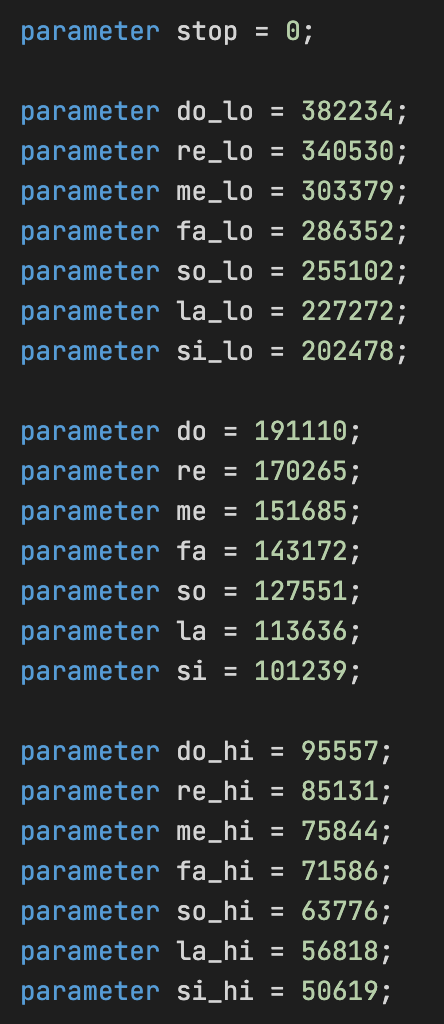
\includegraphics[height=5cm]{fig/music_par}}
	\end{column}%
	
	\centerline{$cnt_{do} \times \frac{1_{sec}}{clk} = \frac{1_{sec}}{freq_{C_4}}$\qquad\quad Parameter $do \approx cnt_{do}$}
\end{frame}

\defverbatim[colored]\musicfreq{
\begin{lstlisting}[language=verilog]
reg [18:0] freq_cnt;

always @ (posedge clk)begin
    if(music_en)begin
        if (freq_cnt >= freq)begin
            freq_cnt = 0;
            music_frac_ext = ~music_frac_ext;
        end
        else
            freq_cnt = freq_cnt + 1;
    end
end
\end{lstlisting}
}

\begin{frame}{Music Player: How does it work?}
	\musicfreq
	\vspace{-2.8em}
	\centerline{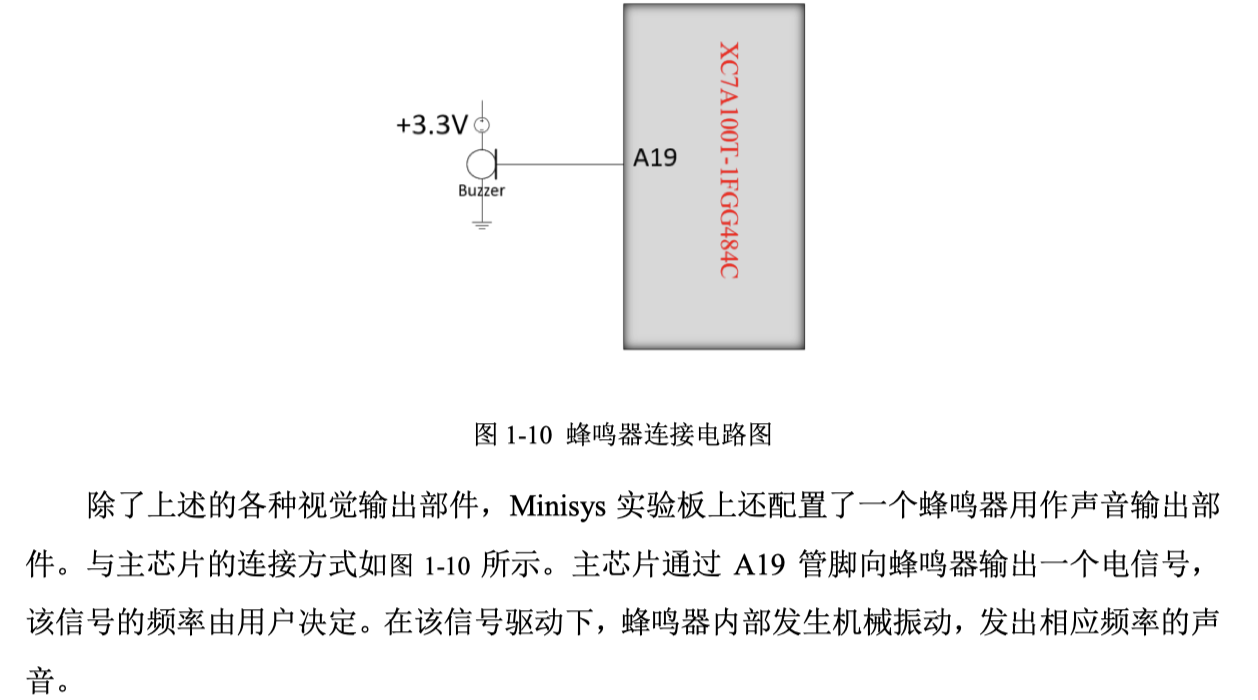
\includegraphics[width=0.56\textwidth]{fig/a19}}
\end{frame}

\defverbatim[colored]\musicread{
\begin{lstlisting}[language=verilog]
always @ (paisp)begin
    if (!music_en)
        freq = stop;
    else begin
        case(song_midi[paisp * 5 +:5])
            'd1    : freq = do_lo;
			// other 20 cases of tones
            default: freq = stop;
        endcase
    end
end
\end{lstlisting}
}

\begin{frame}{Music Player: Encoding music}
	\musicread
	\vspace{-3em}
	\begin{itemize}
		\item<0-> 22 tones: $C_3 \sim B_3$ (lo), $C_4 \sim B_4$ ("Middle C" is $C_4$), $C_5 \sim B_5$ (hi), plus a \textit{stop}.
		\item<0-> $\lceil\log_2 22\rceil =5$, thus in our "musical score", 5 bits are used to represent one beat.
	\end{itemize}
	\vspace{.5em}
	\centerline{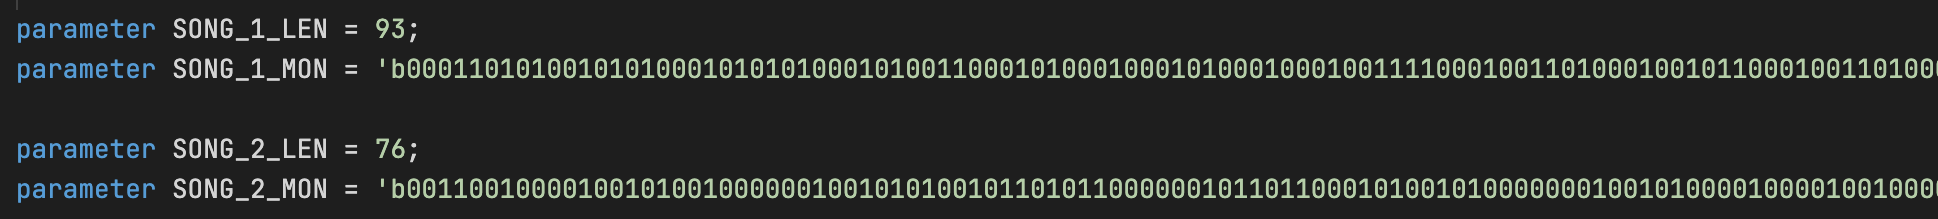
\includegraphics[width=0.86\textwidth]{fig/music_encode}}
\end{frame}

\defverbatim[colored]\musicswitch{
\begin{lstlisting}[language=verilog]
always @ (posedge clk)begin
    if (music_en)begin
        if(paicg >= pai_gap)begin
            paicg <= 0;
            if (paisp == 0)begin
                if(music_rep)
                    paisp = song_len;
            end
            else
                paisp = paisp - 1;
        end
        else begin
            paicg = paicg + 1;
        end
    end
end
\end{lstlisting}
}

\begin{frame}{Music Player: Switching beats}
	\musicswitch
\end{frame}
